\documentclass[a4paper,8pt, twocolumn]{extarticle}
\usepackage[utf8]{inputenc}
\usepackage{graphicx}
\usepackage{tikz}
\usetikzlibrary{arrows,shapes,positioning,snakes}
\usepackage[center]{caption}
\usepackage[english]{babel}
\usepackage[top=2.5cm, bottom=2.5cm, left=2.5cm, right=2.5cm]{geometry}

%---------------------------------------------
% Font packages
%---------------------------------------------
% \usepackage{lmodern}
% \usepackage{concmath}
% \usepackage{cmbright}
% \usepackage{kpfonts}
% \usepackage[adobe-utopia]{mathdesign}
\usepackage{fouriernc}
\usepackage[T1]{fontenc}

%---------------------------------------------
% Tabular package 
%---------------------------------------------
\usepackage{booktabs}
\usepackage{pifont}
\newcommand*\rot{\rotatebox{90}}
\newcommand*\rotsix{\rotatebox{60}}
\newcommand*\OK{\ding{51}}
\usepackage{multirow}
\usepackage{subfig}

%---------------------------------------------
% Math environment packages & command
%---------------------------------------------
\usepackage{amsmath}
\usepackage{amssymb}
\usepackage{array}
% \usepackage{mathrsfs}
\usepackage{array}
% \def\sgn{\mathop{\rm sgn}\nolimits} 
% \usepackage{bbm}


%---------------------------------------------
% item option
%---------------------------------------------
\usepackage{enumitem}
%\setitemize{itemsep=0pt}
\renewcommand{\labelitemi}{-}
%\renewcommand{\itemsep}{2em}

%---------------------------------------------
%HEADER & FOOTER
%---------------------------------------------
\usepackage{fancyhdr}
\pagestyle{fancy}

\renewcommand{\headrulewidth}{.15pt}
\fancyhead[C]{{\textsc{Micro Management in RTS Games}}} 
\fancyhead[L]{Page \thepage \ of \pageref{LastPage}}
\fancyhead[R]{DD2438}

\renewcommand{\footrulewidth}{.15pt}
\fancyfoot[C]{\thepage} 
% \fancyfoot[L]{truc}
% \fancyfoot[R]{bidule}

\usepackage{lastpage}

%---------------------------------------------
% two column option
%---------------------------------------------
\setlength{\columnsep}{0.7cm}


%---------------------------------------------
% Table of content
%---------------------------------------------
\usepackage[colorlinks,linkcolor=black, citecolor=black]{hyperref}

%---------------------------------------------
% Opening
%---------------------------------------------
\title{Artificial Intelligence \& Multi Agent Systems :\\ \textsc{Micro Management in Real Time Strategy Games}}
%\author{Björn \textsc{Holm}, Kilian \textsc{Demeulemeester} \\ \texttt{\{bjh,kiliande\}@kth.se}}
\author{Björn \textsc{Holm} \\ KTH \\ \texttt{bjh@kth.se}
    \and
Kilian \textsc{Demeulemeester} \\ KTH \\ \texttt{kiliande@kth.se}}
\date{\today}

%---------------------------------------------
% Numerotation Handling
%---------------------------------------------
 %\setcounter{section}{3}
 \usepackage[explicit]{titlesec}
  %\titleformat{<command>}[<shape>]{<format>}{<label>}{<sep>}{<before>}[<after>]
	\titleformat{\section}[block]{\normalsize\bfseries\filcenter}{\Roman{section}.}{1em}{#1}
	\titleformat{\subsection}[block]{\normalsize\bfseries}{\emph{\Alph{subsection}.}}{1em}{\emph{#1}}
 %\titleformat{\section}[hang]{\normalfont\Large\bfseries}%
     %{}{8pt}%
     %{\arabic{section}. #1}


%---------------------------------------------
% Dummy text
%---------------------------------------------
\usepackage{lipsum}

%---------------------------------------------
% Bibliography package
%---------------------------------------------
\usepackage{url}
\hypersetup{urlcolor=black}
\usepackage{breakurl}

%---------------------------------------------
% Item package option 
%---------------------------------------------
\newenvironment{shortitem}{
    \begin{itemize}
        \setlength{\topsep}{1ex}
        \setlength{\partopsep}{1ex}
        \setlength{\itemsep}{0ex}
        \setlength{\parskip}{0pt}
        \setlength{\parsep}{1ex}
    }{\end{itemize}}

\newenvironment{enum}{
    \begin{enumerate}
        \setlength{\topsep}{1ex}
        \setlength{\partopsep}{1ex}
        \setlength{\itemsep}{0ex}
        \setlength{\parskip}{0pt}
        \setlength{\parsep}{1ex}
    }{\end{enumerate}}
    

\newenvironment{descri}{
    \begin{description}
        \setlength{\topsep}{1ex}
        \setlength{\partopsep}{1ex}
        \setlength{\itemsep}{0ex}
        \setlength{\parskip}{0pt}
        \setlength{\parsep}{1ex}
    }{\end{description}}

%---------------------------------------------
% Algorithm form
%---------------------------------------------
    \usepackage{amsthm}
    \usepackage{thmtools}
    \declaretheorem[thmbox=M]{algorithm}
%\newtheorem{algorithm}{Algorithm}[section]
\newtheorem{criteria}{Criteria}[section]
\newtheorem{problem}{Problem}
\newtheorem{subproblem}{Problem}[section]
\newtheorem{definition}{Definition}[section]

\begin{document}

% % Indentation size
% \setlength\parindent{0em}
% 
% \setlength{\itemsep}{0pt}

\maketitle

\begin{bfseries} Abstract -- \end{bfseries}
\emph{
Real Time Strategy games (RTS) present a complete simulated environment that pose many interesting challenges to the research of Artificial Intelligence (AI).
Among these challenges are the huge branching factor of play and constrained time for decision.
In this paper we restrict ourselves the management of military troops at a micro-level, that is: given a scenario with for example 10 vs.\ 10 units that have already discovered each other, which actions should our units perform?
}

\emph{
We describe three different approaches: using scripted behaviors, Alpha-Beta search and UCT search, for unit control in combat scenarios in the game Stacraft: Broodwar, using the Broodwar API (BWAPI) for interfacing with the game \cite{BWAPI}.
}


\vspace{0.5cm}
\hrule

%\tableofcontents

\section{Introduction amd Background}
RTS games provide a very interesting platform for developing and testing multi agent coordination.
%In game theoretic terms, RTS games can be considered symmetric, non-zero-sum, simultaneous, imperfect information, combinatorial games.
That which separates RTS games the most from traditional games like chess is the huge branching factor when taking every possible combination of every unit's allowed moves into account, and even in a 10 vs 10 unit battle, all the different ways a battle could play out quickly grows beyond what is feasible to perform an exhaustive search on.
On top of that, a complete model of how the game mechanics work might not be available, and new decisions have to be taken in only the time between each frame
\footnote{
As an example, in the 2011 AIIDE \textsc{Starcraft} AI Competition, 55 ms were given to the bots per frame.
\url{https://skatgame.net/mburo/sc2011/rules.html}
}
.

The game of \textsc{Starcraft} is a good platform for evaluating different methods for addressing these difficulties and several tournaments are held yearly
\footnote{
\url{http://www.sscaitournament.com/}\\ 
\url{http://www.aiide.org/starcraft} \\
\url{http://bots-stats.krasi0.com/} (ladder)
}
.

The game can be roughly divided into two parts, managing the economy (to produce combat units), and managing combat units.
The term \emph{micromanagement} can be used to describe the low-level actions performed by the player in both the economic and the combat aspects of the game, but we will henceforth only refer to it in the context of combat.
For micromanagement, most of current bots such as \emph{UAlbertaBot} and \emph{Skynet}, the two top winning bots in the 2013 AIIDE \textsc{Starcraft} AI competition,
\footnote{\url{http://webdocs.cs.ualberta.ca/~cdavid/starcraftaicomp/report2013.shtml}
}
use scripted behaviors.
Scripted behaviors are usually relatively simple preprogrammed descriptions of what course of action should be taken for a given state of the world, for example, attack the closest enemy.
These algorithms provide good results in term of computational speed but often lack in foresight.
Another approach is to use search-based methods, which naturally adapt to the current situtation.
Looking ahead often allows for finding winning variations where scripted solutions fail because they cannot be preprogrammed to handle every possible state that is in theory winnable.
For reference, in the games of Chess or Go, the problem of finding an optimal winning solution has been proven to be NP-HARD \cite{nphard}.

%\section{Related Work}
%...

However even classical search based method have to be modified in order to take in account simultaneous and non-instaneous moves of RTS games.
In \cite{abcd} a fast search method -- Alpha-Beta search for duratives moves -- is presented and proven better than commonly used AI scripts (with battle up to 8 vs 8 units). 
\cite{wargusuct} investigates the use of UCT -- a Monte-Carlo planning algorithm for this problem -- and provide a battle planning strategy better than several baselines and even a human player.


\section{Scope}
In this paper we only focus of the micro-management of units during combat in RTS games.
The scenario is: there are two players, each is given a number of units at different locations that are relatively close and the whole map is visible. And the goal is to destroy all enemy units, with minimal losses on the own team.
The main challenging questions are:
\begin{enumerate}
        \setlength{\topsep}{0pt}
        \setlength{\partopsep}{0pt}
        \setlength{\itemsep}{0pt}
        \setlength{\parskip}{0pt}
        \setlength{\parsep}{0pt}
    \item How to navigate units? 
    \item How to cooperate well with team members?
    \item How to detect and exploit opponent weaknesses?
    \item How to coordinate attacks?
\end{enumerate}


\section{Model}
The different tasks that have to be accomplished when playing a complete game of Starcraft could be grouped into an hierarchy as in Figure \ref{conceptualModel}. This somewhat captures the way human think about the entities of the game when playing.

\begin{figure}[h!t]
\centering
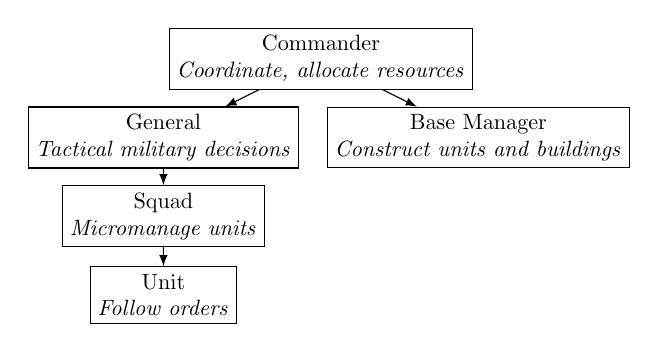
\begin{tikzpicture}[node distance = 1 cm]
    \tikzstyle{quadri}=[rectangle,draw, align=center, scale=0.8]
    \tikzstyle{link}=[->,thin,>=latex]
    \node[quadri] (commander) at (0,2) {Commander \\ \emph{Coordinate, allocate resources}};
    \node[quadri] (general) at (-2,1) {General \\ \emph{Tactical military decisions}};
    \node[quadri] (squad) at (-2,0) {Squad \\ \emph{Micromanage units}};
    \node[quadri] (unit) at (-2,-1) {Unit \\ \emph{Follow orders}};
    \node[quadri] (basemanager) at (2,1) {Base Manager \\ \emph{Construct units and buildings}};
    \draw[link] (commander)--(general);
    \draw[link] (general)--(squad);
    \draw[link] (squad)--(unit);
    \draw[link] (commander)--(basemanager);

\end{tikzpicture}
\caption{
\emph{Conceptual model} of the high level task involved in playing a complete game of Starcraft. All actors in this hierarchy are virtual except for the units.
}
\label{conceptualModel}
\end{figure}

\begin{definition}[Commander]
One per game. Decides how the available resources should be allocated between expanding the base to enable harvesting new resources even faster, and towards producing military units to defend and attack.
\end{definition}
\begin{definition}[Base Manager]
One per game. Constructs what the Commander wants, possibly given priorities.
\end{definition}
\textbf{}\begin{definition}[General]
One per game. Splits the available military units up into squads and assigns them objectives such as \texttt{Attack}, \texttt{Defend} and \texttt{Flee}.
\end{definition}
\begin{definition}[Squad]
As many as the general wants. They have a military goal and micromanage every move of each unit.
\end{definition}
\begin{definition}[Unit]
The actual units in the game, ordered according to the wishes of the squad manager.
\end{definition}


\section{Architecture}

In order to have a huge flexibility in our bot behaviors we designed our AI in a modular and hierarchical fashion (Figure \ref{classDiag}).


\begin{figure}[h!b]
\centering
\begin{tabular}{|c|}
\hline
Commander \\
\emph{Make the overall decision} \\
\hline
\end{tabular} \ \\
\begin{tabular}{c}
$\downarrow$
\end{tabular} \ \\
\begin{tabular}{|c|}
\hline
Squad Manager \\
\emph{Handle $n$ units and lead them into battle} \\
\hline
\end{tabular} \ \\
\begin{tabular}{c}
$\downarrow$
\end{tabular} \ \\
\begin{tabular}{|c|}
\hline
Units \\
\emph{Fight for glory} \\
\hline
\end{tabular}
\caption{Class Diagram}
\label{classDiag}
\end{figure}

Our bot also uses behaviors tree (using the library in \cite{libbehavior}). A example of the behavior tree used by the units acheiving \texttt{Kitting\footnote{Staying at a distance, using ranged attacks, and running whenever the enemy comes near}} is depicted in Figure \ref{behaAttackClos}.

\begin{figure}[h!b]
\caption{Behavior tree for kitting}
\label{behaAttackClos}
\end{figure}

Two differents behaviors has been study for our bot:
\begin{shortitem}
\item Scripted based behaviors
\item Heuristic based behaviors
\end{shortitem}

\begin{definition}[Scripted based behaviors]
Make decision only on a reactive way and do not make any plan for the future of the game.
\end{definition}

\begin{definition}[Heuristic based behaviors]
% TODO
blabla...
\end{definition}

\section{Kiting}

Kiting behavior is worth more explanation. 
We based our algorithm on the work of\:\cite{kiting}. 

\begin{definition}[Kiting]
    Kiting (to kite) is to move units around to make the enemy chase them and thus not be able to attack as much, or not at all. 
    Kiting can be summarize as:
    \begin{shortitem}
    \item Move out of range
    \item Turn back and shoot at the enemy
    \item Repeat
    \end{shortitem}
\end{definition}

The behavior tree used by the units acheiving \texttt{Kiting} is depicted in Figure \ref{behaAttackClos}.

\begin{figure}[h!t]
\centering
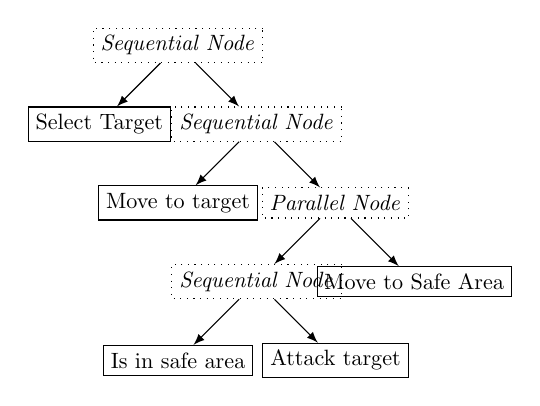
\begin{tikzpicture}[node distance = 1 cm]
    \tikzstyle{leaf}=[rectangle, align=center, scale=0.8, draw]
    \tikzstyle{node}=[rectangle,dotted, align=center, scale=0.8, draw]
    \tikzstyle{link}=[->,thin,>=latex]
    \node[node] (start) at (1,4) {\emph{Sequential Node}};

    \node[leaf] (target) at (0,3) {Select Target};
    \node[node] (seqNode) at (2,3) {\emph{Sequential Node}};

    \node[leaf] (leafMove) at (1,2) {Move to target};
    \node[node] (paraAttack) at (3,2) {\emph{Parallel Node}};

    \node[node] (attackNode) at (2,1) {\emph{Sequential Node}};
    \node[leaf] (moveSafe) at (4,1) {Move to Safe Area};

    \node[leaf] (isSafe) at (1,0) {Is in safe area};
    \node[leaf] (attack) at (3,0) {Attack target};

    \draw[link] (start)--(target);
    \draw[link] (start)--(seqNode);

    \draw[link] (seqNode)--(leafMove);
    \draw[link] (seqNode)--(paraAttack);

    \draw[link] (paraAttack)--(attackNode);
    \draw[link] (paraAttack)--(moveSafe);

    \draw[link] (attackNode)--(attack);
    \draw[link] (attackNode)--(isSafe);
\end{tikzpicture}
\caption{Behavior tree for kiting}
\label{behaAttackClos}
\end{figure}

When selecting the target our bot try to select a target on which a kiting strategy can be used (for instance unit \texttt{A} can not kite another unit \texttt{A}). 
If it can not find any kitable unit then a classic attack is perform (\emph{fight to the death while standing on your position}).

As in paper \cite{kiting} the kiting bot uses an influence map for performing kiting: a 2D matrix $I_{enemy}$.

Let $e$ be an enemy. $e$ has an influence of the area $(i,j)$ of the map if the area can be reached by the enemy before performing kiting.
This relation is denoted $e \textasciitilde (i,j)$.

\begin{multline*}
    e \textasciitilde (i,j) \Leftrightarrow \\ d(e,(i,j)) \leq e.attackRange + e.speed * kitingTime
\end{multline*}

Then the influence matrix is define as:
$$
I_{enemy}(i,j) = \sum_{e \textasciitilde (i,j)}e.DPS  
$$

Using this matrix each unit can compute its closest safe position.

Then an attack is performed each time the unit is in a safe area.



\section{Game Combat Model}

In order to execute search of a solution, we created a model based on the work of \cite{abcd}, composed of the following components:

\begin{definition}[State]
A state $s=<t,p,m,U>$ is composed of the following:
\begin{shortitem}
\item Current game time $t$
\item Player $p$ who performed action $a$ to generate $s$
\item 
\end{shortitem}
\end{definition}

\begin{definition}[Unit]
a
\end{definition}

\begin{definition}[Action]
a
\end{definition}

\begin{definition}[Effect]
a
\end{definition}



\section{Search}

Our goal is to implement search algorithm based on the graph generated by our model. 
We focused on two differend algorithm: UCT (Upper Confident Bound) and ABCD (Alpha-Beta Considering Durations).  
It is well known that a good child ordering in a game tree graph can greatly improve performances.  
If better child are searched first, Alpha-Beta can produce better cuts and search deeper and UCT search will spend less time exploring less valuable moves. 
The time restriction of RTS game is transposed in term of graph exploration as a maximum number of child and/or depth limitation. 
This idea is reffered as \emph{move ordering} in \cite{portfolio}.
Their main idea behind move ordering is to consider first actions that would be produced by scripted behaviors.

\subsection{UCT Search}
UCT, or Upper Confidence bound for Trees, is the most popular Monte Carlo Tree Search algorithm for playing games that are otherwise hard for computers to handle.
This algorithm has recently seen success in the game of go, but more relevant to our topic, also been applied to games such as Arimaa, and even RTS games. For a review of how it works we refer to \cite{mcts}.
Arimaa is interesting because it has an average branching factor of 17000, compared to chess, which only has 35. \cite{arimaawiki}

In \cite{wargusuct}, UCT is used for deciding where squads should attack in the RTS game Wargus, which would correspond to using UCT at the General-level in our conceptual model as well.

\subsection{ABCD Search}
In \cite{abcd}, an extended version of alpha-beta pruning, which is a well-known searching algorithm, was used for micro-management. 
They were able to find good solutions for 8 v.s. 8 unit scenarios in 5 ms, achieving around a 80\% win rate against their best script.

The evaluation functions suggested by \cite{abcd} are the following:
\begin{shortitem}
\item Straight Forward Evaluations:
$$
    \displaystyle{SFE(s) = \sum_{u \in U_1} u.hp - \sum_{u \in U_2} u.hp } 
$$

\item Life Time Damage:
$$
    \displaystyle{LTD(s) = \sum_{u \in U_1} u.hp \cdot u.DPF- \sum_{u \in U_2} u.hp \cdot u.DPF } 
$$

\item Life Time Damage 2:
$$
    \displaystyle{LTD2(s) = \sum_{u \in U_1} \sqrt{u.hp} \cdot u.DPF - \sum_{u \in U_2} \sqrt{u.hp} \cdot u.DPF } 
$$
\end{shortitem}

Where $DPF$ in the damage per frame of a unit (see section \ref{kiting}), $U_1$ (resp. $U_2$) is the set of player's (resp. opponent's) units .

$SFE$ doesn't take into account unit strike force -- which is an essential information during a battle. 
$LFD$ present a good estimation of this strike force but do not favour having a greater number of units. 
Ultimately $LTD2$ measure the strike force and favor the greatest number of units remaining\footnote{Having two units with $50$ hit points gives more power than one with $100$ hit points.}.

In order to use alpha-beta algorithm it is necessary to separates the player's actions and its opponents action.
It can be done quiet efficiently by considering the children of a node as the restriction of its children to only one player set of actions:
$$
S_{A|p} = \{A \in S_A | \forall a \in A, a \text{ is an action performed by $p$}\}
$$
Algorithm \ref{algABCD} presents the ABCD algorithm.
The main disctinction with the ``classic'' alpha-beta algorithm is that there is not a perfect alternation between $MAX$ and $MIN$. Once a state has no possible actions, we move in time until an action can be performed for one of the player. 
Figure \ref{figABCD} shows an exemple of such a graph: once we've reached a state where no action can be made for both player, we advance in time. In this new frame, there is an action for $MAX$. Therefore it is still him who is considered as the current player.

\begin{figure}[h!t]
    \begin{algorithm}[ABCD (Alpha-Beta Considering Durations)]
Let $s_0$ be the root node, $MAX$ be the player and $MIN$ the opponent. The algorithm return the best move compute by $ABCD(s_0,d_{max},-\infty,+\infty,MAX)$ where: \ \\

        \textbf{Function} $ABCD(s,d,\alpha,\beta,p)$:
        \begin{enum}
        \item \textbf{If} ($s$ is a terminal state) \textbf{Return} $LTD2(s)$
        \item \textbf{Else}
            \begin{enum}
            \item If $S_{A|p} \neq \emptyset$ 

            \begin{enum}
            \item \textbf{While} $S_{A|p} \neq \emptyset$
                \begin{enum}
                \item Pop $s_1$ from $S_{A|p}$ 
                \item Let $v = ABCD(s_1,d-1,\alpha,\beta,\bar{p})$
                \item \textbf{If} $p = MAX$ and $(v > \alpha)$ \textbf{then} $\alpha = v$
                \item \textbf{If} $p = MIN$ and $(v < \beta)$ \textbf{then} $\beta= v$
                \item \textbf{If} $\alpha \geq \beta$ \textbf{then break} 
                \end{enum}
            \item \textbf{Return} $(p = MAX) ? \alpha : \beta$ 
            \end{enum}
        \item \textbf{Else if} $S_{A|\bar{p}} \neq \emptyset$
            \begin{enum}
            \item \textbf{Return} $ABCD(s,d,\alpha,\beta,\bar{p})$
            \end{enum}
        \item \textbf{Else} 
            \begin{enum}
            \item Advance in time to state $s'$ for which $S'_A \neq \emptyset$
            \item \textbf{Return} $ABCD(s',d,\alpha,\beta,p)$
            \end{enum}
        \end{enum}
        \end{enum}
        \ \\
        And $s$ being considered as a \textbf{terminal state} if $d_{max}$ is reached, the time is elapsed or the state is a winning/loosing situation.
        \label{algABCD}
    \end{algorithm}
\end{figure}

\begin{figure}[h!t]
\centering
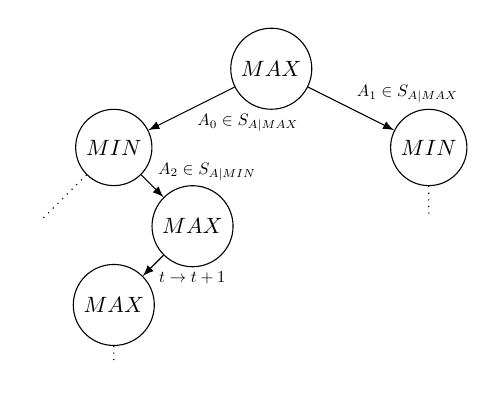
\begin{tikzpicture}[node distance = 1cm]
    \tikzstyle{node}=[circle,align=center,scale=0.8,draw]
    \tikzstyle{nodenotgen}=[circle,dotted,align=center,scale=0.8,draw]
    \tikzstyle{nodeterm}=[circle,fill=gray!30,align=center,scale=0.8,draw]
    \tikzstyle{link}=[->,thin,>=latex]
    
    \node[node] (s0) at (4,4) {$MAX$};

    \node[node] (s1) at (2,3) {$MIN$};
    \node[node] (s3) at (6,3) {$MIN$};

    \node[auto,scale=0.8] (s33) at (6,2) {};
    \draw[-,>=latex,dotted] (s3) to (s33);

    \node[auto,scale=0.8] (s4) at (1,2) {};
    \node[node] (s6) at (3,2) {$MAX$};

    \node[node] (s7) at (2,1) {$MAX$};

    \node[auto,scale=0.8] (s8) at (2,0.2) {};
    
    \draw[link] (s0) to node [auto,scale=0.6] {$A_0 \in S_{A|MAX}$} (s1); 
    \draw[link] (s0) to node [auto,scale=0.6] {$A_1 \in S_{A|MAX}$} (s3);
    \draw[-,>=latex,dotted] (s1) to (s4);
    \draw[link] (s1) to node [auto,scale=0.6] {$A_2 \in S_{A|MIN}$} (s6);
    \draw[link] (s6) to node [auto,scale=0.6] {$t \rightarrow t+1$} (s7);
    \draw[-,>=latex,dotted] (s7) to (s8);
    

\end{tikzpicture}
    \caption{Exemple of a graph constructed by the ABCD-algorithm}
    \label{figABCD}
\end{figure}


\section{Results}

At the present time our micromanagement bots need more development (UCT search) and/or more testing. This part will be accomplished in a future work.

So far all of the testing has been made by testing our bot against the built-in AI of \textsc{Starcraft}. While not sure of how this AI work it seems to pack all unit together and send them in a suicide mission (move to closest target, attack it, repeat). 

This AI is able to defeat the \texttt{Attack Closest} bot on almost every game (10 vs 10 often leads to 3--4 man standing for the opponent team).
Indeed, \texttt{Attack Closest} do not present any cooperative work neither fleeing behavior for in danger units. However, \texttt{Attack Closest Lethal} defeat the AI on almost every game with a ration of \textasciitilde25\% of player units still alive. This bot offers a very good cooperation between unit.

Since kiting behavior can not be tested with the same kind of units we tested it by fighting slow powerful but low range units (\texttt{zealot}) versus fast long range units (\texttt{Vulture}). 
In that situation our bot was able to defeat the opponent team almost every time (even in scenario such as 3 (us) VS 10 (opponent)). 
Theoretically, one unit should be enough. However the bot attack sequence sometimes gets stuck in attack mode (our bot was unable do detect that the attack has been performed) and therefore the \texttt{Vulture} unit is destroyed almost instantly by the \texttt{Zealots}.


\vspace{0.5cm}
\hrule
\vspace{0.5cm}
\begin{bfseries} Conclusion -- \end{bfseries}
    \emph{While extremely complicated in term of searchability, RTS game are indeed a solid platform for developing and testing multi agent cooperative behaviors. Our work was focused on micro management and we were able to implement some ``classic behaviors'' (\emph{i.e} behaviors used by real human player).} 
    \emph{We also manage to create a model which can be used in most RTS game. The game state representation can easily be extender in order to take in account more kind of unit, more effect, etc.} 
\emph{Even if the search algorithms did not defeat the built-in AI, the results are encouraging. Improving move ordering and find unit group abstractions that reduce the state space are good lead in order to improve them.}
\emph{We have to keep in mind that the ultimate goal of this line of research is to handle large combat scenarios in real time -- where scripted behaviors shows their weaknesses.}


\nocite{*}
\bibliographystyle{plain}
\bibliography{bibliography}

\end{document}
